% !TeX root = main.tex
\chapter{Introduction \label{ch1-intro}}

The following chapter is a description for using Latex. The most basic steps will be explained including citation, adding figures, making tables, ... and so on. If you have already used Latex before or are familiar with the process, this chapter might not be interesting for you. But if you are new to the concept or need a refresher, the following might be useful to you.

Not everything might be apparent if you are reading this text as a PDF-file. For further understanding, read the actual latex-file (go to 01-chapters/ch1-intro.tex).

\section{Getting started with Latex}

If you haven't worked with Latex yet, you first have to install a few things. Go to the README.md file and follow the instructions.

\section{Add a new chapter}

To add a new chapter, right-click on 01-chapters and add a new document. In order for it to be displayed in your PDF-file, it first has to be included. Go to main.tex and include it, as shown.


\section{Including figures}

The command to include a graphic is "\textbackslash includegraphics". To add a description use the following command "\textbackslash caption\{your Text\}". However this command can only be used in a specific surrounding (marked by "\textbackslash begin\{figure\}" and "\textbackslash end\{figure\}".

The surrounding has also other functions, which you can use; for futher information look up the following website: \url{https://de.overleaf.com/learn/latex/Inserting_Images}


\begin{figure}[ht]
	\centering
	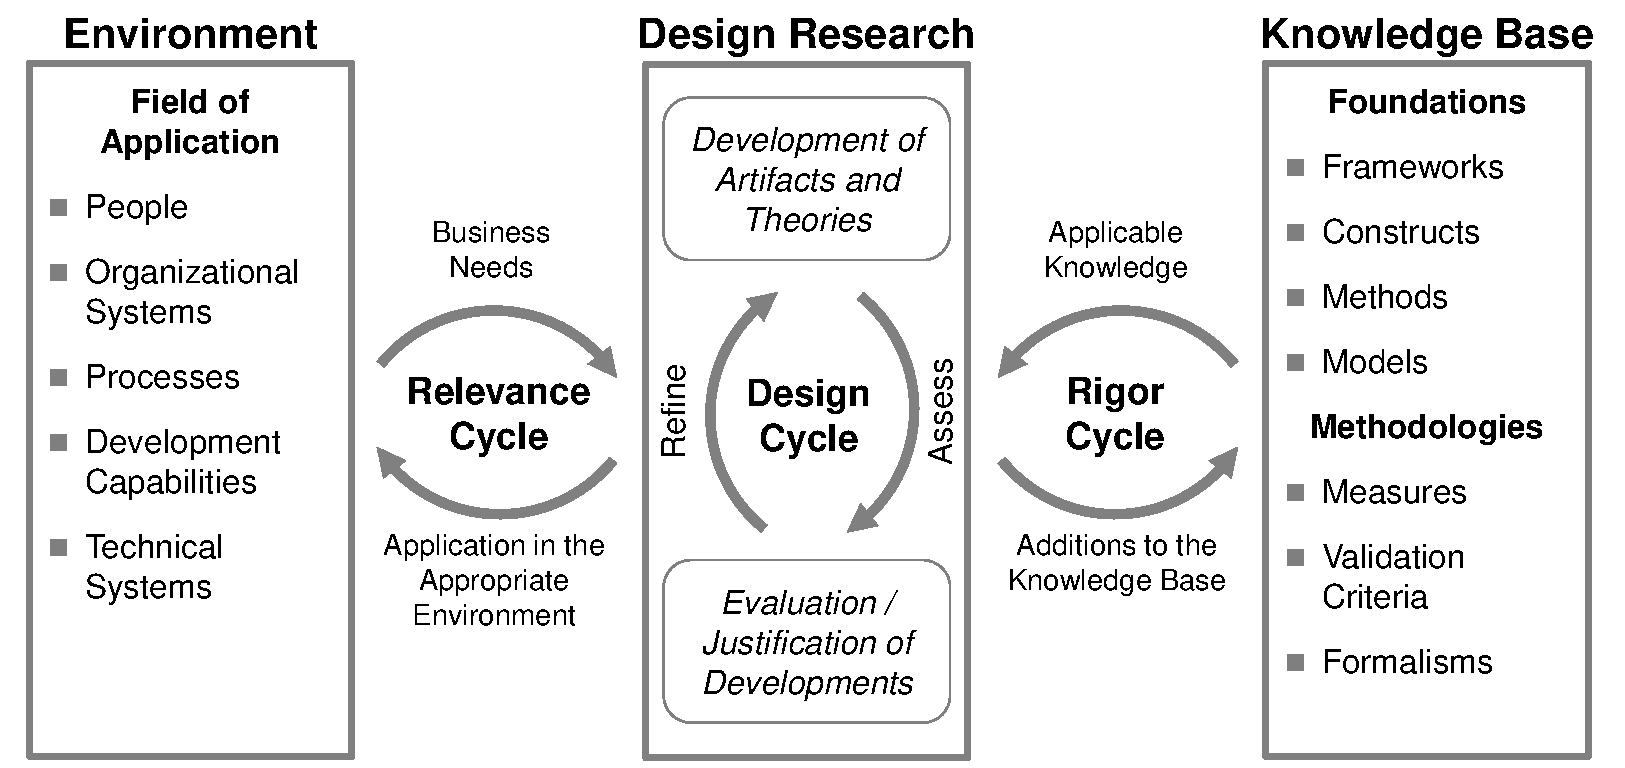
\includegraphics[width=1\textwidth]{DSR}
	\caption{TMP: Design science research framework original image \cite[based on][p. 80]{HEVN04}.}
	\label{fig:DSR}
\end{figure}



\section{Including tables}

The compilation of a table can be difficult, especially if everything needs to be consistent. In order to simplify this task, try using the following website: \url{https://www.tablesgenerator.com/}
It provides a simple user interface, which generates the table for you.

The "label"-command is for referencing the table or graphic in your text: Table \ref{desserts}.

\begin{table}[H]
    \caption{Comparison of different desserts.}
    \label{desserts}
    \centering
    \begin{tabular}{@{}lllll@{}}
        \toprule
        hier soll was stehen & gut & neutral & schlecht & k.A. \\ \midrule
        Käsekuchen           &     &         &          &      \\
        Schokotorte          &     &         &          &      \\
        Brombeereis          &     &         &          &      \\ \bottomrule
    \end{tabular}
\end{table}



\section{Citation}

In order to cite a reference, it first has to be included to the Bib. To do so, follow the instructions of the following link: \url{https://www.youtube.com/watch?v=kbvf01ExKVU}


\section{Acronyms}

For adding something to the Acronyms, go to "en" or "de" (depending on you using german or english) and select "frontmatter.tex". In this document you will find the table of Acronyms.
